%% ----------------------------------------------------------------
%% SETTINGS
%% ----------------------------------------------------------------
\documentclass[../et.tex]{subfiles}

%% ----------------------------------------------------------------
%% BEGIN
%% ----------------------------------------------------------------
\begin{document}

%% ----------------------------------------------------------------
%% DOCUMENT
%% ----------------------------------------------------------------
Para diseñar la interfaz del usuario en la PC, se decidió utilizar el lenguaje de programación Python, por su simplicidad y cantidad de librerías y recursos que se pueden encontrar en línea.

Esta app fue dividida en dos, el backend que se comunica con el microcontrolador y la interfaz gráfica utilizando la librería Tkinter. Esta librería fue elegida por su simplicidad y ya que viene incluida por defecto en Python.

En la \autoref{fig:software} se puede ver una imagen de la ventana principal. Se utiliza una barra superior, donde se puede elegir el puerto COM, refrescar la lista de puertos, conectarse al dispositivo y ver su estado; una barra lateral, donde se muestran y modifican parámetros; y la ventana principal, donde se puede elegir el test a correr y ver su resultado.

\begin{figure}[!htbp]
    \centering
    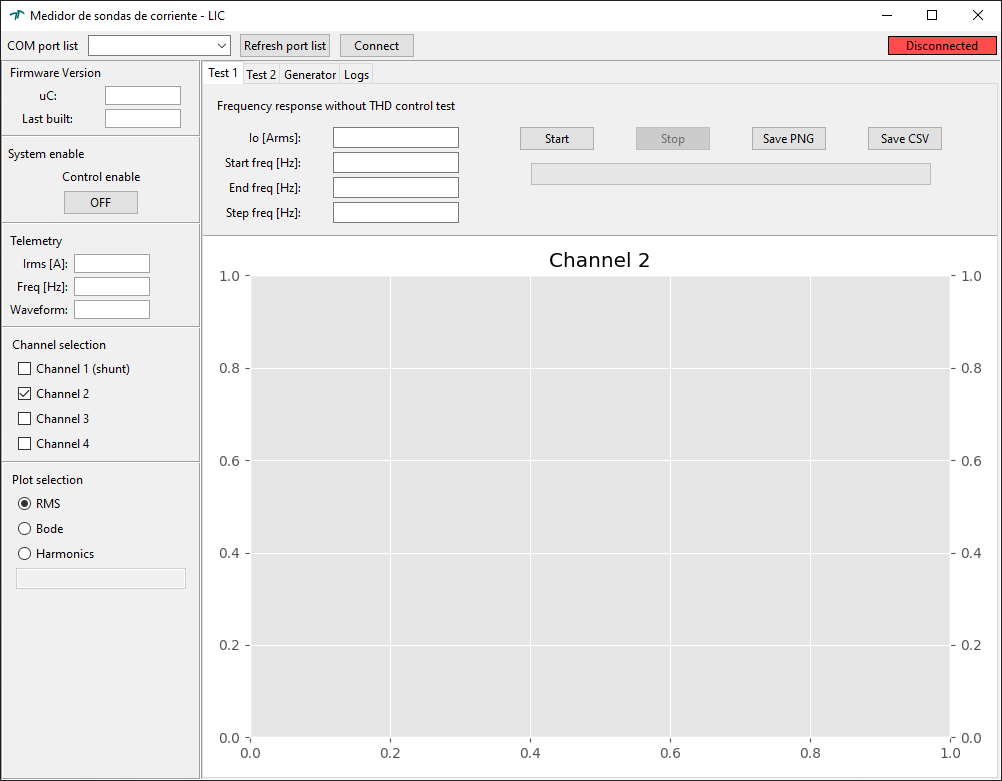
\includegraphics[scale=0.6]{../images/software-gui.png}
    \caption{Ventana principal interfaz PC}
    \label{fig:software}
\end{figure}

En cada uno de estos tests se podrá guardar un informe en formato PNG o CSV, si se necesita trabajar con esos datos crudos. Además, se pueden ver los logs del sistema, seleccionando el nivel de profundidad con el que se quiere inspeccionar.

\textit{To be continued...}


\end{document}
